%!TeX encoding=UTF-8
%!TeX root=main.tex
%!TeX program=xelatex

\documentclass[aspectratio=169,dvipsnames]{beamer}

\usetheme[sectionpage=progressbar,subsectionpage=progressbar,numbering=fraction,
          progressbar=foot]{metropolis}

\graphicspath{{../img/}}
\usepackage{svg}
\svgpath{{../img/}}

\usepackage{appendixnumberbeamer}

\usepackage{hyperref}

\usepackage{datetime}
\newdate{defensedate}{27}{06}{2018}
\newdate{startdate}{07}{02}{2018}
\newdate{enddate}{22}{06}{2018}

\usepackage[cache=false,newfloat]{minted}
\usepackage{inconsolata}
\setmonofont{Inconsolata}
\newfontfamily\DejaSans{DejaVu Sans}

\usepackage{textcomp}

\usepackage{xpatch}
\usepackage[citestyle=authortitle,backend=bibtex]{biblatex}
\addbibresource{../bibl.bib}
\xapptobibmacro{cite}{\setunit{\nametitledelim}\printfield{year}}{}{}
\renewcommand{\footnotesize}{\scriptsize}

\title{Adapting Amplified Unit Tests for Human Comprehension\\\large{Internship --- M2 SIF}}
\subtitle{Supervisor: Benoit Baudry\\KTH, Sweden\\\displaydate{startdate}--\displaydate{enddate}}

\date{\displaydate{defensedate}}
\author{%
  Simon Bihel\hfill\href{mailto:simon.bihel@ens-rennes.fr}{\nolinkurl{simon.bihel@ens-rennes.fr}}\\
}
\institute{%
  University of Rennes I \\
  \'Ecole Normale Sup\'erieure de Rennes
}


% 20 minutes + 5 minutes for questions

\begin{document}

\maketitle


\section{Introduction}

\begin{frame}{Test Suites}
  \metroset{block=fill}
  \begin{block}{Context}
    \begin{itemize}
      \item Software projects are now accompanied by strong test suites
      \item Takes time to write
      \item Still missing some bugs due to focus on nominal paths when writing test cases
    \end{itemize}
  \end{block}

  \pause{}

  \begin{block}{Related works}
    \begin{itemize}
      \item Measure the quality of test suites
      \item Automatically write test suites
      \item \alert{Amplify} existing test suites
    \end{itemize}
  \end{block}
\end{frame}

\begin{frame}{Concepts}
  System-Under-Test: function, class, whole program\dots
  \begin{description}
    \item[Inputs] E.g.\ function parameters, method calls to setup and stimulate an object
    \item[Assertions] Used to test whether the function's output is correct, that the object is in the right state
  \end{description}
\end{frame}
\begin{frame}[fragile]{Test Example}
  \vspace*{-1em}
  \begin{minted}[linenos,breaklines,highlightlines={4,6,8},highlightcolor=YellowOrange!20]{java}
public class TreeListTest {
    @Test
    public void testIterationOrder() {
        TreeList tl = new TreeList(10);
        for (int i = 0; i < 10; i++) {
            tl.add(i);
        }
        ListIterator it = tl.listIterator();
  \end{minted}
  \begin{minted}[linenos,breaklines,firstnumber=last,highlightlines={12},highlightcolor=YellowGreen!20]{java}
        int i = 0;
        while (it.hasNext()) {
            Integer val = it.next();
            assertEquals(i++, val.intValue());
        }
    }
}
  \end{minted}
\end{frame}

\begin{frame}{Metrics for Test Suites}
  \begin{columns}
    \begin{column}{0.75\textwidth}
      \metroset{block=fill}
      \begin{block}{Goal}
        Detect parts that are not tested.
      \end{block}

      \pause{}

      \begin{exampleblock}{Code Coverage}
        Number of instructions or branches executed by the test suite.
      \end{exampleblock}

      \pause{}

      \begin{exampleblock}{Mutation Testing}
        \begin{enumerate}
          \item Create \emph{mutants} (i.e.\ bugged versions) of the main software (e.g.\ change a \texttt{>} with a \texttt{<=}).
          \item Count how many mutants for which the test suite fail.
        \end{enumerate}
      \end{exampleblock}
    \end{column}
    \begin{column}{0.25\textwidth}
        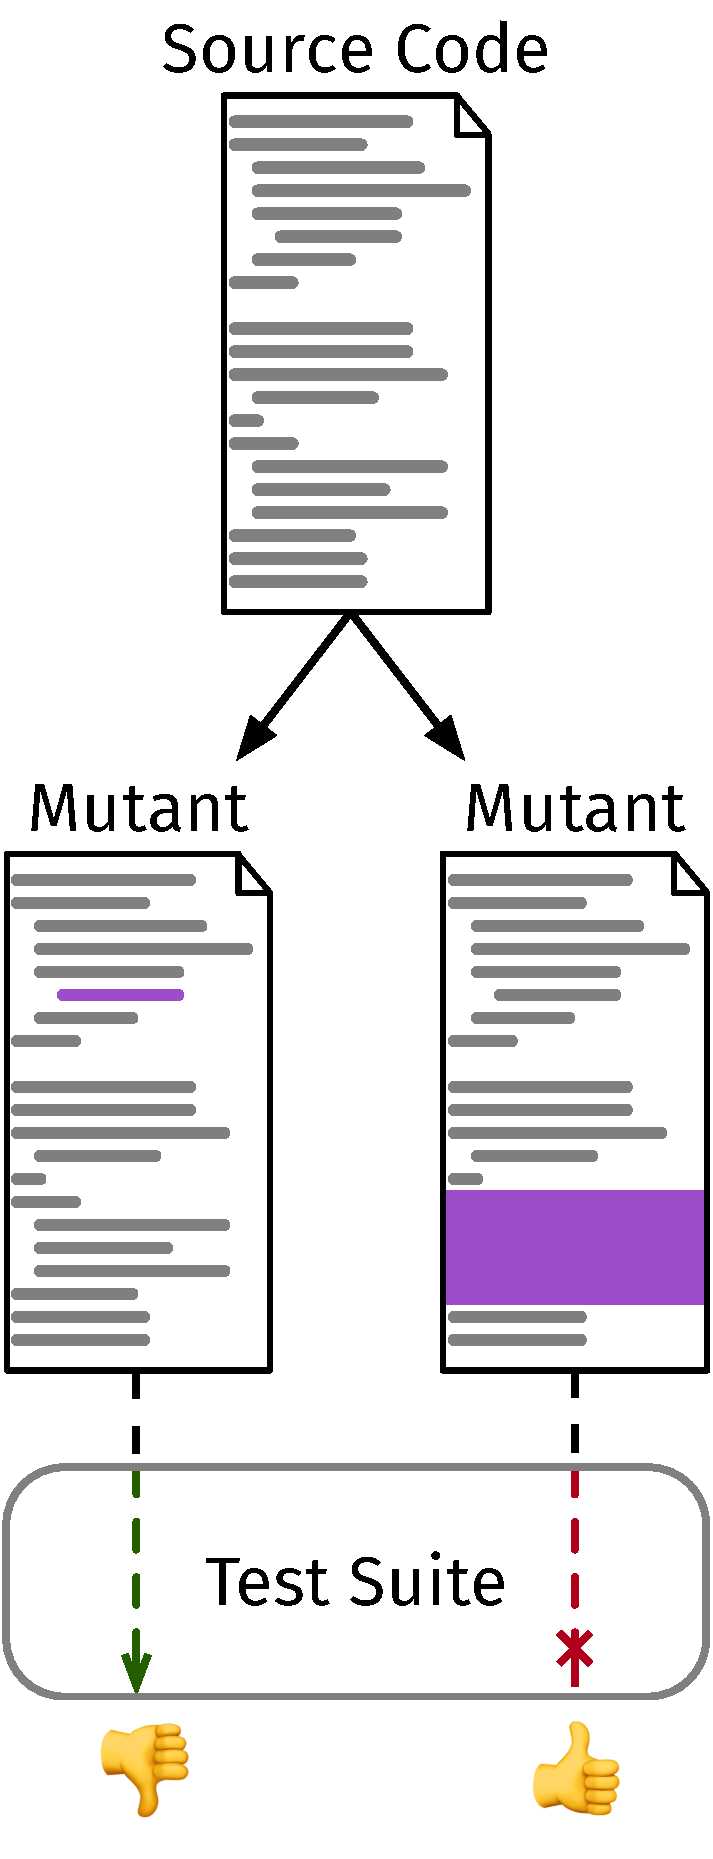
\includegraphics[height=\textheight]{mutation_testing}
    \end{column}
  \end{columns}
\end{frame}

\begin{frame}{Automated Test Generation}
  \metroset{block=fill}
  \begin{block}{Goal}
    Generate tests from scratch to fulfill a given metric.

    Large search space of instructions and values.
  \end{block}

  \begin{exampleblock}{Search-based techniques~\footcite{mcminn2011search}}
    Random, iterative and heuristic-based techniques (e.g.\ Genetic Algorithms, simulated annealing).
  \end{exampleblock}

  \pause{}

  \begin{block}{The oracle problem~\footcite{barr2015oracle}}
    What should the output of a test be?

    \textrightarrow{} Avoid this by focusing on regression testing.
  \end{block}
\end{frame}


\section{Test Suite Amplification}

\begin{frame}{Motivations~\footcite{danglot2017emerging}}
  \begin{itemize}
    \item Reduce search-space by using the existing test suite as a (good) starting population.
    \item Use knowledge in hand-written tests for a better oracle.
  \end{itemize}
\end{frame}

\begin{frame}{DSpot~\footcite{baudry2015dspot}}
  \metroset{block=fill}
  \begin{block}{Goal}
    Create tests for undetected mutants.
  \end{block}
  \begin{center}
    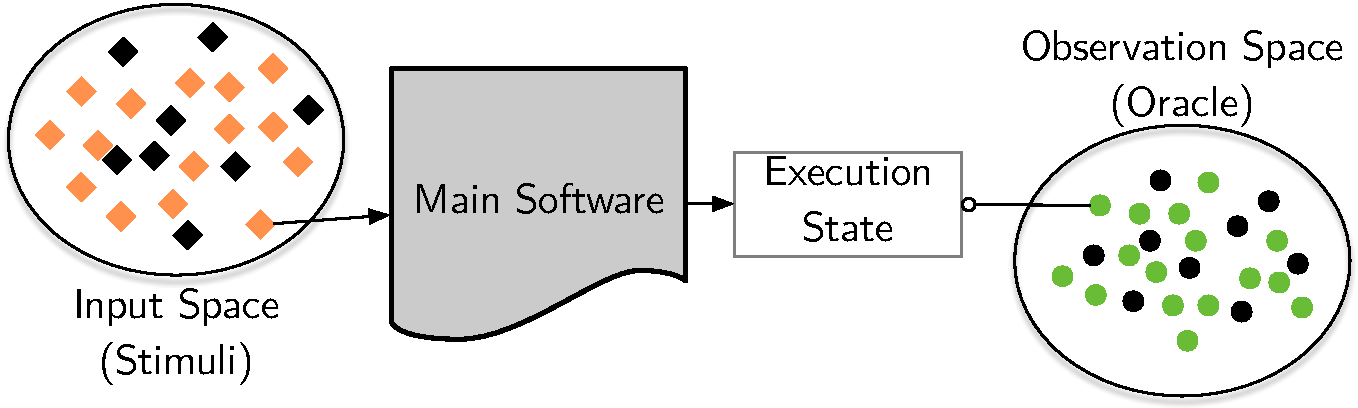
\includegraphics[scale=0.5]{spaces_report}
  \end{center}
\end{frame}

\begin{frame}{DSpot --- Amplification Operators}
  \metroset{block=fill}
  \begin{block}{Input amplification}
    \textbf{Literals \textrightarrow{}} replaced with neighbor values.

    \textbf{Method calls \textrightarrow{}} duplicated, removed or made-up (with random or default parameters).
  \end{block}

  \vfill
  \pause{}

  \begin{block}{Assertion amplification}
    Capture the state of the system after the test's execution.
  \end{block}
\end{frame}

\begin{frame}{Usage in the DevOps Context}
  \begin{center}
    \alert{New tests ought to be approved by the developers.}
  \end{center}
\end{frame}


\section{Generating Descriptive Messages}

\begin{frame}{Related Works}
  \begin{center}
    \textbf{\Large{Software Artefact Summarization}}\footcite{nazar2016summarizing}
  \end{center}

  Includes: documentation for source code, code changes, \alert{test cases}.

  \vfill{}
  \pause{}

  \metroset{block=fill}
  \begin{block}{Example}
    \begin{itemize}
      % \item<+-> Classification of test cases.\footcite{li2018automatically}
      \item<+-> \textit{UnitTestScribe}\footcite{li2016automatically} Summarises actions in natural language.
    \end{itemize}
  \end{block}
\end{frame}

\begin{frame}{Contribution}
  \begin{center}
    Pull Request message.
  \end{center}

  Explain:
  \begin{enumerate}
    \item the modifications made,
    \item the reason why the new test was kept (i.e.\ mutation score).
  \end{enumerate}
\end{frame}

\begin{frame}{Logging Amplifications}
  \begin{description}
    \item[Category] \texttt{ASSERT}, \texttt{ADD}, \texttt{DEL}, \texttt{MODIFY}
    \item[Parent] Type of the parent of modified AST node.
    \item[Role] Role for the parent node (e.g.\ argument for a method call).
    \item[Old value] Textual representation of the old node.
    \item[New value] Textual representation of the new node.
  \end{description}

  \pause{}

  250 ELoC.

  Logging call in each amplifier.
\end{frame}

\begin{frame}{Mutation Score Information}
  \begin{description}
    \item[Location] Modified method and line.
    \item[Description] High-level, sometimes vague, natural language description from PIT\footcite{coles2016pit}.
  \end{description}
\end{frame}

\begin{frame}{Target Platform}
  \begin{center}
    
\includegraphics[width=8em]{markdown-logo}

    Markdown markup language allows for enhanced messages.
    Code snippet, links to code lines, better rendering, \dots
  \end{center}

  Major platforms use it.
  
\includegraphics[width=9em]{GitHub_Logo}
  
\includegraphics[width=9em]{wm_no_bg}

  \vfill{}

  But not all.
  
\includegraphics[width=9em]{Bitbucket-blue}
\end{frame}

\begin{frame}{Message Generator}
  655 Python ELoC.

  \href{https://github.com/sbihel/xwiki-commons/issues/2\#issuecomment-394699634}{Demo XWiki}
\end{frame}

\begin{frame}{Evaluation}
  \metroset{block=fill}
  \begin{block}{Performances}
    Logging:
    \begin{itemize}
      \item no impact on time,
      \item 6\% higher memory usage.
    \end{itemize}

    Few seconds for the message generation.
  \end{block}

  \pause{}

  No case study with users. Only discussions with my supervisor.
\end{frame}


\section*{Conclusion}

\begin{frame}{Summary}
  \metroset{block=fill}
  \begin{block}{Too early to tackle the topic of generated tests explanation.}
    \begin{itemize}
      \item Lack of precise information (e.g.\ killed mutants \textit{per} test).
      \item Small user-base.
    \end{itemize}
  \end{block}

  \pause{}

  \begin{block}{What I should have focused solely on.}
    \begin{itemize}
      \item Cleaning amplified tests.
      \item Independent mutation score explanation.
    \end{itemize}
  \end{block}
\end{frame}

\appendix

\begin{frame}[standout]

\end{frame}

\begin{frame}
  \begin{center}
      
\includegraphics[width=0.5\textwidth]{evosuite-logo}\footcite{fraser2011evosuite}
  \end{center}
  \begin{itemize}
    \item Test Suite Generation \emph{from scratch}.
    \item State-of-the-Art \& industry grade.
  \end{itemize}

  \vfill

  \metroset{block=fill}
  \begin{block}{Differences}
    \begin{itemize}
      \item Treats test suites as a whole.
      \item GA with tests cases as genes.
    \end{itemize}
  \end{block}

  \begin{block}{Automatic Documentation}
    Automatic name generation\footcite{daka2017generating}.
  \end{block}
\end{frame}

\begin{frame}{Is Documentation Essential? --- Yes.}
  Developers surveys\footcite{daka2014survey,prado2015wap,prado2016advances,prado2018towards,li2016automatically} and experiments\footcite{panichella2016impact}.

  Documentation (e.g.\ JavaDoc, naming) has many advantages\footcite{daka2017generating}, especially for generated tests\footcite{rojas2017search,shamshiri2018how}:
  \begin{itemize}
    \item faster to get familiar with the test;
    \item faster fault localisation; and
    \item helps to build trust in a test generator if it can provide a proof for its result.
  \end{itemize}
\end{frame}

\end{document}
